\section{Capacitati de comunicare in rețea utilizand Android}

\subsection{Afisarea informatiilor despre interfetata de retea WiFi}
Pentru a afisa informatii despre interfata de retea WiFi a dispozitivului, trebuie sa folosim clasa \textit{WifiManager}.
Aceasta clasa ne ofera acces la informatii pentru toate aspectele legate de conectivitatea WiFi.
Deoarece aceasta clasa este un serviciu de sistem, trebuie sa obtinem o referinta la aceasta folosind metoda \textit{getSystemService()}.
\begin{lstlisting}[language=Kotlin]
    val wifiManager = this.context?.getSystemService(Context.WIFI_SERVICE) as WifiManager;
\end{lstlisting}
Aceasta clasa contine o proprietate numita \textit{connectionInfo} care ne ofera informatii despre conexiunea WiFi curenta.
\begin{lstlisting}[language=Kotlin]
    val wifiInfo = wifiManager.connectionInfo;
\end{lstlisting}
Daca am apela metoda \textit{toString()} pe acest obiect, am obtine un sir de proprietati separate de virgula.
\begin{lstlisting}[language=Kotlin]
    SSID: "AndroidWifi", BSSID: 00:13:10:85:fe:01, MAC: 02:00:00:00:00:00, IP: /10.0.2.16, Security type: 0, Supplicant state: COMPLETED, Wi-Fi standard: 1, RSSI: -50, Link speed: 1Mbps, Tx Link speed: 1Mbps, Max Supported Tx Link speed: 11Mbps, Rx Link speed: 2Mbps, Max Supported Rx Link speed: 11Mbps, Frequency: 2447MHz, Net ID: 0, Metered hint: false, score: 60, isUsable: true, CarrierMerged: false, SubscriptionId: -1, IsPrimary: -1, Trusted: true, Restricted: false, Ephemeral: false, OEM paid: false, OEM private: false, OSU AP: false, FQDN: <none>, Provider friendly name: <none>, Requesting package name: <none>"AndroidWifi"openMLO Information: , Is TID-To-Link negotiation supported by the AP: false, AP MLD Address: <none>, AP MLO Link Id: <none>, AP MLO Affiliated links: <none>
\end{lstlisting}
Schimband virgulele cu caractere de linie noua, le putem afisa intr-un TextView.
\subsubsection{Afisarea informatiilor in interfata grafica}
\subsubsection{Rezultat}

Ruland programul folosind emulatorul, putem observa informatiile afisate in interfata grafica.

\begin{figure}[H]
    \centering
    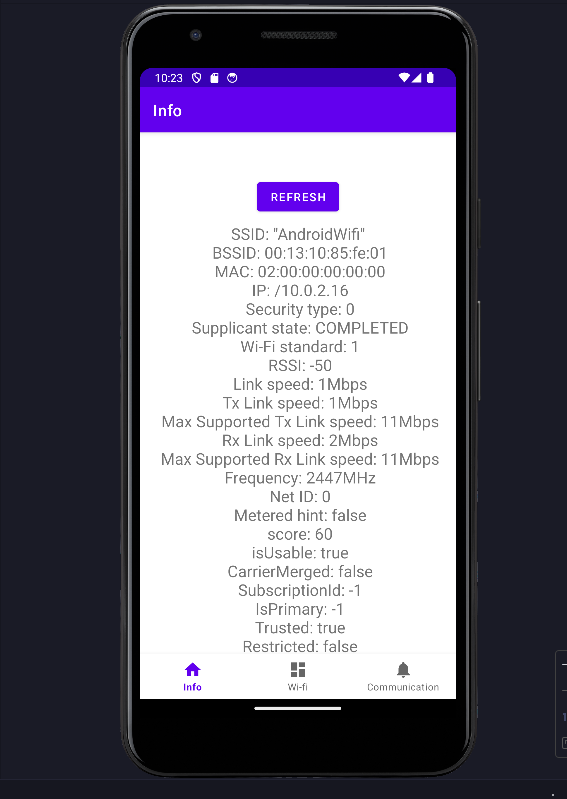
\includegraphics[width=0.7\linewidth]{figs/wifi_info_emulator.png}
    \caption{Informatii despre reteaua WiFi ruland aplicatia in emulator}
    \label{fig:wifi_info}
\end{figure}

Putem observa ca informatiile afisate par a fi "dummy" si nu sunt reale. Acest lucru se datoreaza faptului ca emuleaza o reteta WiFi si un dispozitiv.
Ruland aplicatia pe un telefon fizic putem observa informatii reale despre reteaua WiFi la care este conectat dispozitivul.